\documentclass[tikz,border=2pt]{standalone}
\usepackage{amsmath,amssymb}
\usetikzlibrary{arrows.meta}
\begin{document}
% (Q,r) = (4,2) policy, demands 2,3,1,4,0,3,2,5,1,2 in periods 1..10, P_1 = 6.
% Each period shows the start position P_k (left half) and the end position P_k' (right half).
% When P_k' <= r = 2 the policy orders the smallest multiple of Q = 4 that brings the position back
% into {r+1,...,r+Q} = {3,4,5,6} (shaded): one lot at the starts of periods 3, 5, 7, two lots (8) at period 9.
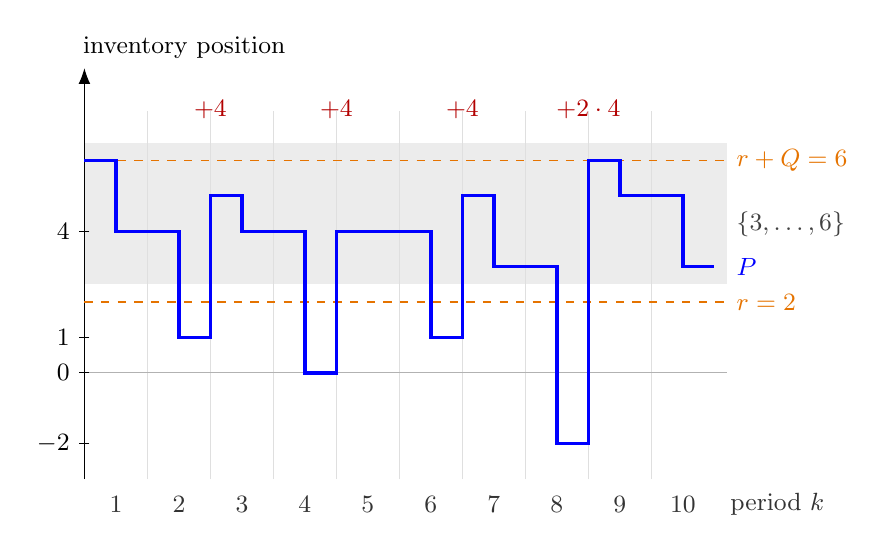
\begin{tikzpicture}[font=\small, >={Latex[length=2mm]}, x=0.8cm, y=0.45cm]
  \fill[gray!15] (0,2.5) rectangle (10.2,6.5);
  \foreach \k in {1,...,9} {\draw[gray!25] (\k,-3) -- (\k,7.4);}
  \draw[gray!60] (0,0) -- (10.2,0);
  \draw[->] (0,-3) -- (0,8.6) node[anchor=south west, xshift=-4pt] {inventory position};
  \foreach \v in {-2,0,1,4} {\draw (0.08,\v) -- (-0.08,\v) node[left] {$\v$};}
  \foreach \k in {1,...,10} {\node[gray!40!black] at (\k-0.5,-3.7) {$\k$};}
  \node[gray!40!black, anchor=west] at (10.1,-3.7) {period $k$};
  % policy levels
  \draw[orange!90!black, thin, dashed] (0,6) -- (10.2,6) node[right] {$r+Q=6$};
  \draw[orange!90!black, thin, dashed] (0,2) -- (10.2,2) node[right] {$r=2$};
  \node[gray!50!black, anchor=west] at (10.2,4.2) {$\{3,\dots,6\}$};
  % position path
  \draw[blue, very thick] (0,6) -- (0.5,6) -- (0.5,4) -- (1,4) -- (1.5,4) -- (1.5,1) -- (2,1) -- (2,5) -- (2.5,5) -- (2.5,4) -- (3,4) -- (3.5,4) -- (3.5,0) -- (4,0) -- (4,4) -- (4.5,4) -- (5,4) -- (5.5,4) -- (5.5,1) -- (6,1) -- (6,5) -- (6.5,5) -- (6.5,3) -- (7,3) -- (7.5,3) -- (7.5,-2) -- (8,-2) -- (8,6) -- (8.5,6) -- (8.5,5) -- (9,5) -- (9.5,5) -- (9.5,3) -- (10,3);
  \node[blue, anchor=west] at (10.2,3) {$P$};
  % orders in lots of Q = 4
  \foreach \x/\q in {2/4,4/4,6/4,8/2\cdot4} {\node[red!70!black, anchor=south] at (\x,6.9) {$+\q$};}
\end{tikzpicture}
\end{document}
